%\documentclass[12pt,letterpaper,margin=0.75in]{article}
%\documentclass[12pt]{article}

\documentclass[12pt, onecolumn]{IEEEtran}

\usepackage[utf8]{inputenc}
\usepackage{amsmath}
\usepackage{amsfonts}
\usepackage{amssymb}
\usepackage{graphicx}
\author{George Engel\\
IC Design Research Laboratory\\
Southern Illinois University Edwardsville\\
}
\usepackage{geometry}

\geometry{
 letterpaper,
% total={8.5in,11in},
 left=1.0in,
 right=1.0in,
 top=1.0in,
 bottom=1.0in,
 }

\usepackage{filecontents}
\usepackage[noadjust]{cite}

\begin{filecontents*}{bibi.bib}
@ARTICLE{507173,
author={Simpson, M.L. and Young, G.R. and Jackson, R.G. and Xu, M.}, 
journal={Nuclear Science, IEEE Transactions on}, 
title={A monolithic, constant-fraction discriminator using distributed R-C delay line shaping}, 
year={1996}, 
volume={43}, 
number={3}, 
pages={1695-1699}, 
keywords={CMOS logic circuits;RC circuits;delay lines;detector circuits;discriminators;monolithic integrated circuits;nuclear electronics;20 mV to 2 V;N-well process;constant-fraction shaping;delay line;distributed R-C delay line shaping;monolithic CMOS constant-fraction discriminator;monolithic constant-fraction discriminator;slope degradation;timing errors;CMOS process;Capacitors;Circuits;Computational fluid dynamics;Delay lines;Detectors;Feedback;Laboratories;Signal generators;Timing}, 
doi={10.1109/23.507173}, 
ISSN={0018-9499}, 
month={Jun},} 
\end{filecontents*}

\title{A Multi-Channel Discriminator IC}

\begin{document}

% Insert title

\maketitle

% INTRODUCTION

\section*{Introduction}

\noindent
This paper attempts to describe a preliminary design for a multi-channel discriminator chip. The integrated circuit (IC) will be called DISC16C, short for discriminator chip - 16 channels. Discriminators are widely used in radiation monitoring systems.  The purpose of a discriminator is to mark the arrival time of an input pulse. Ideally, the discriminator's output logic signal, marking the arrival of the input pulse, should be independent of pulse amplitude and risetime.

\noindent
\newline
In reality, variations in the firing time of a discriminator generally fall into two categories: time walk, $t_w$, and time jitter, $\sigma_t$. The term time "walk" is used to describe systematic variation in the rising edge of the discriminator output signal as a function of pulse height and time "jitter" describes random variation in the rising edge of the output signal due to electronic noise in the system.\\  

\section*{Design Specifications}
\noindent

\begin{itemize}
\item
Support 16 detectors.
\item
Must support pulses of both polarities.
\item
Must accommodate signals with risetime constants ranging from 3 nsec to 100 nsec.
\item
Should exhibit excellent walk and jitter characteristics for input pulse amplitudes ranging from 20 mV to 2 V. 
\item
Must accommodate pulse repetition rates up to 1 KHz.
\item
The discriminator in each of the 16 channels should be of the constant fraction type (CFD). In CFD discriminators an attenuated version of the input is subtracted from a delayed version of input waveform and the time at which the difference between the two is equal to zero is used to mark the pulse arrival time. This results in output timing signals independent of pulse amplitude.
\item
Each channel should have a leading-edge threshold. The threshold is programmed using a 4-bit digital value.
\item
While the chip must support signals with risetime constants ranging from 3 nsec to 100 nsec, performance will be optimized for the shorter time constants. 
\item
The output pulse width from a channel will be programmable (through an external analog control voltage) in the range of 10 nsec to 100 nsec.
\item
The analog supply voltage for the IC will be 5 Volts while all digital signals entering and leaving the IC will obey a 3.3 Volt standard.
\item
Power consumption of the 16 channel IC should not exceed 350 mW \emph{i.e.} 20 mW per channel with 30 mW budgeted for the circuits common to all channels. 
\item
The IC is expected to occupy an area of aprpoximately 4 mm x 3 mm.  The chip will be packaged in a 64-pin plastic package.  A ground pin be be placed between the 16 analog input pins in order to reduce crosstalk.
\item
The chip is to be fabricated in the ON Semiconductor, 0.5 micron CMOS process.  The targeted process supports two poly and 3 metal layers.  A high resistance poly layer is available.
\end{itemize} 
 
\section*{System Level Design Description}
\noindent
The design presented herein is similar to the discriminator circuit currently being used in our group's HINP4 IC which in turn is based on a design described in \cite{507173}. The design presented in \cite{507173} describes a design carried out in 1.2 micron CMOS and boasts timing walk for 5 ns risetime signals over the dynamic range from 20 mV to 2 V of less than $\pm$ 150 ps.  The reported jitter was 10 ps with an input level of 20 mV.

\noindent
\newline
A block diagram depicting a single channel of our proposed multi-channel discriminator IC is presented in Fig.~\ref{BlockDiagram}. The leading edge discriminator circuit shown in the figure consists of a cascade of 2 or 3 very high bandwidth (but relatively low gain) differential amplifiers. A "slow" DC offset cancellation loop drives the input referred offset for the cascaded amplifier to the sub-mV level. The amplified (offset-free) output is then compared with a programmable threshold using a continuous-time comparator.  The output from the leading edge circuit qualifies the output from the zero-cross circuit.  The leading edge comparator transitions first followed by the firing of the zero-cross discriminator, thereby accurately marking input pulse arrival time. \\

\begin{figure}[htbp!]
	\centering
 	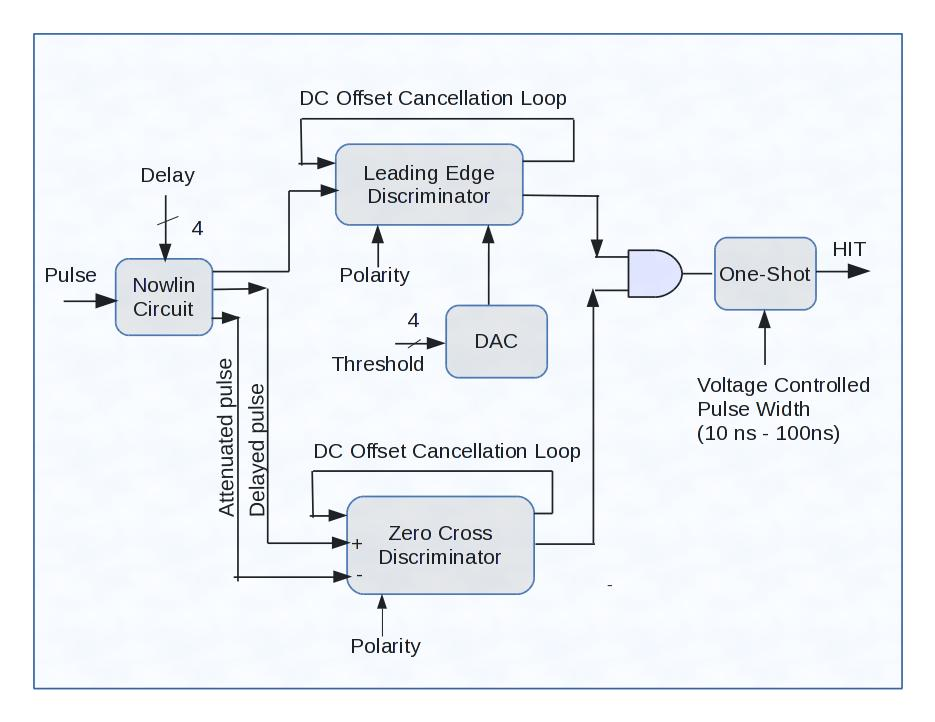
\includegraphics[scale=0.5,keepaspectratio=true]{./images/DISC16block.jpg}
 	\caption{Leading edge circuit qualifies output of zero-cross discriminator.  Leading edge and zero-cross circuits consists of a cascade of low-gain, high-bandwidth simple differential amplifiers driving a very high gain-bandwidth product (GBW) comparator }
 	\label{BlockDiagram}
\end{figure}

\noindent
The Nowlin circuit is shown in greater detail in Fig.~\ref{Nowlin}.  The capacitor $C_0$ in the Nowlin cicuit along with the series resistance of $R_1$ and $R_2$ implement a "fast" shaper.  The output of this highpass filter is applied to the leading edge discriminator. Also, a fraction, $(\frac{R_2}{R_1 + R_2})$, of the "fast" shaper output is applied to the inverting input of the zero-cross discriminator circuit along with a delayed version of the input pulse connected to the non-inverting input. It is well-known that the time at which the differential voltage crosses through zero is independent of the input pulse amplitude.\\

\begin{figure}[htbp!]
	\centering
 	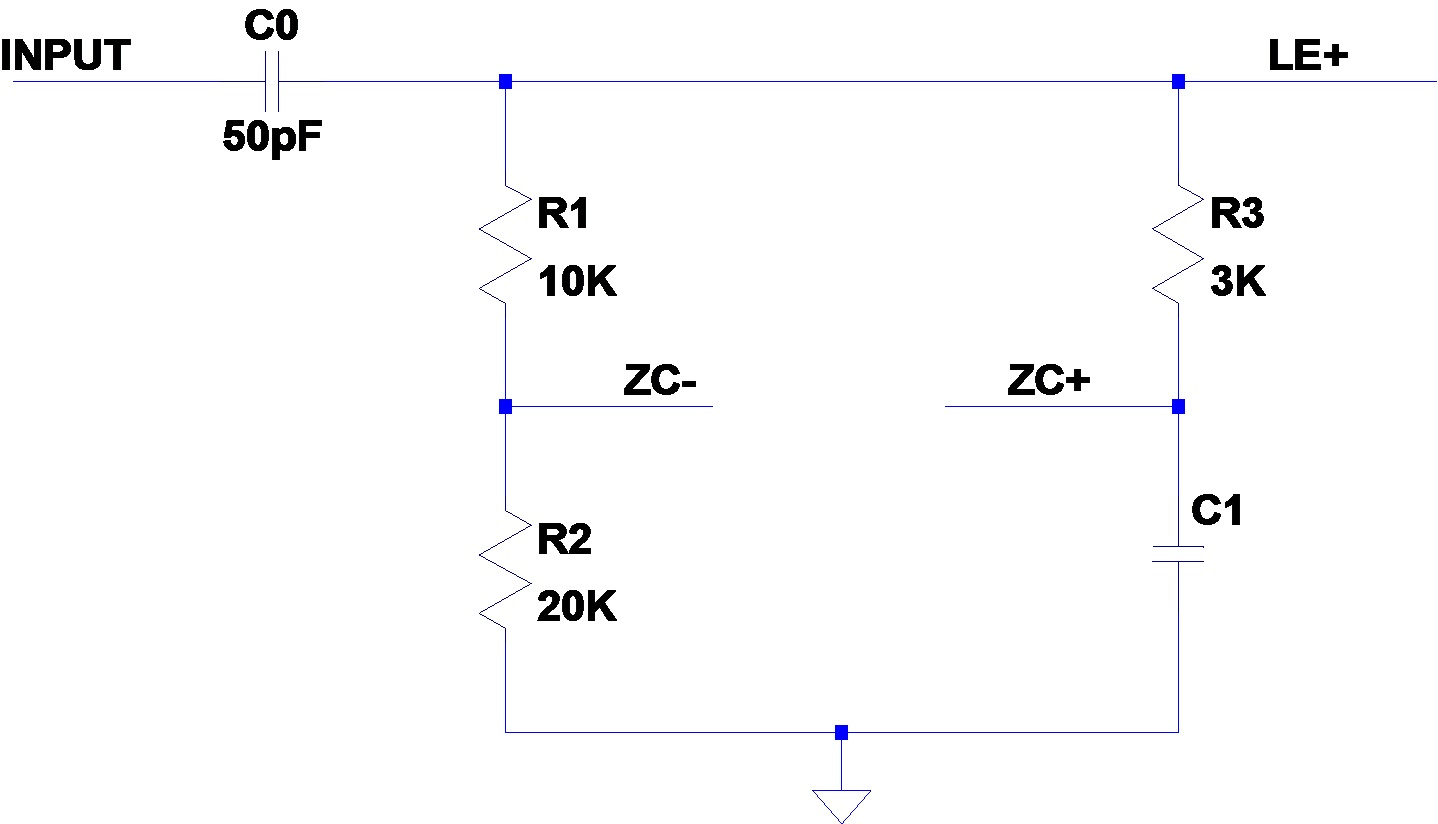
\includegraphics[scale=0.3,keepaspectratio=true]{./images/nowlin.jpg}
 	\caption{Nowlin circit using lumped components, $R_3 \text{ amd } C_1$, to implement delay. Here the fraction is $\approx$ 0.7.}
 	\label{Nowlin}
\end{figure}

\noindent
It is important that the slope (which we shall refer to as the "slew rate" or SR) of the differential signal when crossing through zero be maximized.  A delay (determined by the time constant $R_3 \cdot C_1$) which when very short will produce maximum SR but at the expense of underdrive voltage. In Fig.~\ref{TypicalWaveforms} the input pulse risetime constant is 3 ns (in other words,  a 10 - 90 \% rise time of 6.6 ns).  When the time constant in the Nowlin circuit is 300 ps, the SR is high but the underdrive is quite small. The underdrive must be sufficiently large so as to drive the comparator output to the logic false state.  Remember, that Fig.~\ref{TypicalWaveforms} remains essentially unchanged when the peak pulse amplitude is reduced to 20 mV except all amplitudes are 1 \% of the values shown in the figure. When the time constant in the Nowlin circuit is 6 ns, the underdrive voltage is high but the SR suffers. Clearly, when the time constant is 1.5 ns, a good compromise between SR and underdrive voltage is achieved. In the proposed design, capacitor $C_1$ and/or resistor $R_3$ will be programmable. In this way, the delay can be matched to the risetime of the input pulse and we can accommodate a wide range of input rise time constants. \\

\begin{figure}[htbp!]
	\centering
 	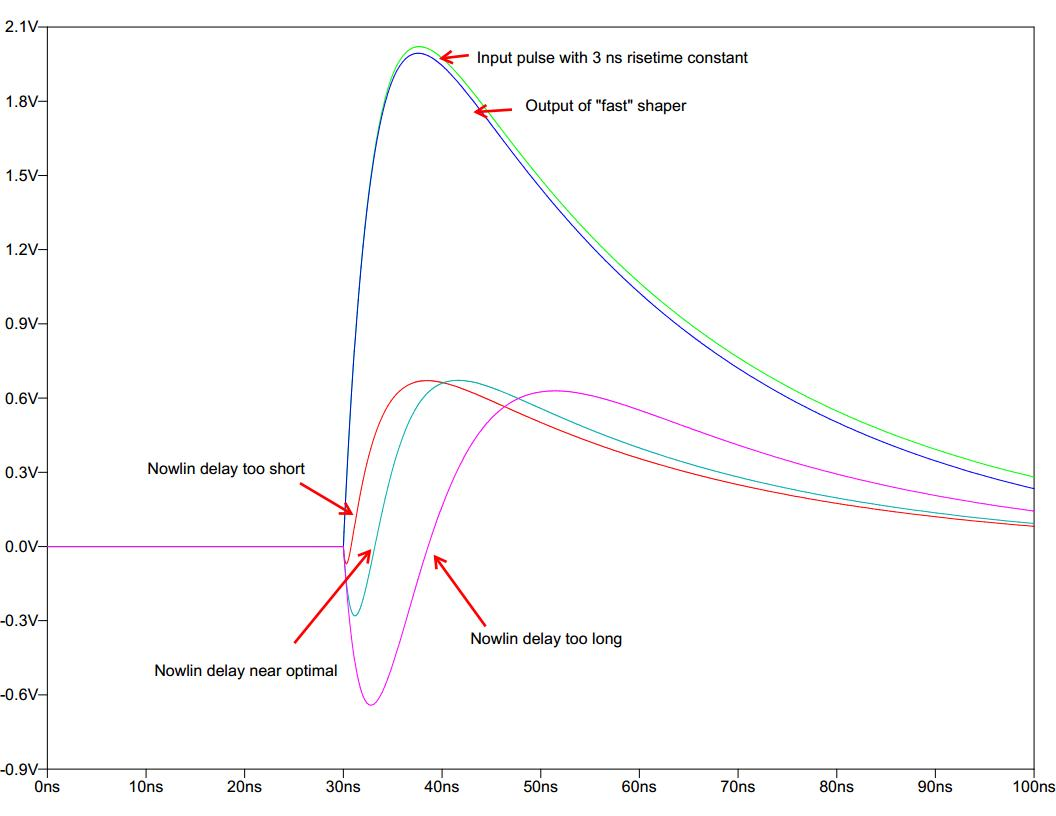
\includegraphics[scale=0.6,keepaspectratio=true]{./images/nowlin_fast.jpg}
 	\caption{Input signal with 3 ns risetime constant. A programmable delay allows matching of the delay provided by the Nowlin circuit to the risetime constant of the input signal.}
 	\label{TypicalWaveforms}
\end{figure}

\noindent
\newline
The zero-cross circuit is constructed by cacading N differential amplifier stages (N $\approx$ 6) each possessing a very wide bandwidth, but relatively low-gain (4X - 7X) with the final output stage driving a very fast analog comparator.  The purpose of cascading a relatively large number of high bandwidth gain stages is to force linear operation where delay is independent of amplitude.  In short, the cascaded amplifier serves as a SR enhancer.  For a first-order system, it is well-known that if the input risetime is not to be severely degraded, the bandwidth, BW, of the amplifier must obey the following equation\\

\begin{equation*}
	BW > \frac{0.35}{t_{10-90}} \approx \text{ 50 MHz}
\end{equation*}

\noindent
\newline
Since we are cascading N stages, the BW of each stage must be increased by $\sqrt{N} \approx 2.5$ resulting in a differential amplifier bandwidth of 125 MHz if the overall BW is to be 50 MHz.  If the stage gain, G, is 5 then the GBW of a single differential amplifier stage needs to be around 625 MHz, clearly achievable in 0.5 micron CMOS.


\section*{Jitter and Time Walk Analyses}

\noindent
For an input pulse with a risetime constant of 3 nsec, we require that \\

\begin{itemize}
\item
the walk not exceed +/- 150 ps over the entire 2 mV - 2 V input amplitude range,
\item
and the jitter should not exceed 300 ps at an input level of 2 mV.
\end{itemize}

\noindent
\newline
We analyze jitter first.  Jitter is a consequence of the electronics noise associated with the Nowlin circuit as well as the noise of the \emph{first} differential amplifier in the zero-cross discriminator circuit (where we assume the noise of succeeding stages when referred to the input is negligible).\\

\noindent
Time jitter can be estimated by taking the total integrated noise at the output of the Nowlin circuit and then dividing by the SR.

\begin{equation*}
\sigma_t = \frac{\sigma_v}{SR}
\end{equation*}


\noindent
\newline
From Fig.~\ref{TypicalWaveforms}, one observes a SR of $200 \frac{V}{\mu s}$ when the input pulse amplitude is 2 Volts.  Because of the exponential nature of the input signal, SR is proportional to pulse amplitude but inversely proportional to the input risetime constant, $\tau_r$. In other words, when the pulse amplitude is reduced to 20 mV, the SR is $2 \frac{V}{\mu s}$. If $\tau_r$ is 30 ns rather than 3 ns, then SR will go down by a factor of ten.  A conservative estimate of total integrated noise, $\sigma_v$, at the output of the Nowlin circuit is $200 \text{ } \mu V$.  Table~\ref{JitterTable} below summarizes the expected jitter performance of the proposed IC.\\


\begin{table}[htbp!]
\begin{center}
\begin{tabular}{||c | c | c | c||} 
\hline
Amplitude (V) & $\sigma_t$ ($\tau_r = 3 ns$) (ps) & $\sigma_t$ ($\tau_r = 15 ns$) (ps) & $\sigma_t$ ($\tau_r = 100 ns$) (ps) \\ [0.5ex] 
\hline\hline
2.0 & 1 & 5 & 33\\ 
\hline
0.2 & 10 & 50 & 330  \\
\hline
0.02 & 100  & 500  & 3300\\ [1ex] 
\hline
\end{tabular}
\end{center}
\caption{Time jitter as function of pulse amplitude and risetime constant.}
\label{JitterTable}
\end{table}

\noindent
We analyze time walk next.  Time walk is is used to describe systematic variation in the rising edge of the discriminator output signal as a function of pulse height.  If we assume a single-pole response for the analog comparator with a gain-bandwidth-product of $GBW_c$, it is not difficult to show that the variation in propagation delay, $\Delta t_{pd}$, due to input pulse amplitude is 

\begin{equation*}
\Delta t_{pd} \approx  \sqrt{\frac{V_{DD}}{2 \cdot \pi \cdot GBW_c \cdot G^N \cdot SR_{min}}}
\end{equation*}

\noindent
\newline
where $V_{DD}$ is the supply voltage, G is the gain of a single differential amplifier stage, N is the number of stages, and $SR_{min}$ is  the SR with a pulse amplitude of 20 mV.   Table~\ref{WalkTable} summarizes the expected walk performance (over the dynamic range of 2 mV - 2 V) for three representative risetime constants.\\

\noindent
In reality, the time walk may increase at low amplitudes because of residual offset.  Ultimately, how well the discriminator performs at low amplitude will depend on the effectiveness of the dynamic offset cancellation loop, shown in Fig.~\ref{BlockDiagram}.  It can be shown that residual offset alters the time at which one crosses zero as given by

\begin{equation*}
\Delta t_{cross} \propto  \tau_r \cdot (\frac{V_{os}}{A})
\end{equation*}

\noindent
where $V_{os}$ is the residual input referred offset and A is the amplitude of the input pulse. It is important that the residual offset be driven to the sub-mV level.  The "slow" DC offset cancellation loop has to be "slow" enough so as not to interfere with the pulse as it passes through the zero-cross discriminator but yet fast enough so that pulse repetition rates as high as 1 kHz can be accommodated.  This will require significant design effort but is certainly feasible, as demonstrated in \cite{507173}. The wide range of pulse risetime constants we wish to support makes this problem more difficult but not impossible.

\begin{table}[htbp!]
\begin{center}
\begin{tabular}{||c | c||} 
\hline
$\tau_R$ (ns) & Time Walk  (ps)\\ [0.5ex] 
\hline\hline
3 & $\pm$ 160 \\ 
\hline
15 & $\pm$ 360  \\
\hline
100 &  $\pm$ 920 \\ [1ex] 
\hline
\end{tabular}
\end{center}
\caption{Time walk as function of risetime constant, $\tau_r$ for $G = 5$, $N = 6$ and $GBW_{c} = 250 MHz$.}
\label{WalkTable}
\end{table}

\section*{Timeline}

\noindent
A timeline for the major development tasks is presented in Fig.~\ref{Timeline}. A top-down design strategy will be employed.  Behavioral simulations written in MATLAB will be used to validate the design specifications and to develop an effective and stable DC offset cancellation loop for both the zero and leading edge circuits.  This will be followed by drawing a complete set of schematics for the IC using Cadence's Virtuoso Schematic Editor. A VerilogA behavioral description will be developed for each of the circuit symbols. After successful simulation of this behavioral description each VerilogA block will be replaced with a transistor level description. As the transistor level descriptions are validated, they will committed to physical layout and verification.  Extensive simulations on the parasitically extracted netlist will be performed before submitting the IC for fabrication. Upon returning from fab, a prototype system will be constructed.  A small number of systems will then be constructed and distributed to interested users. The success of the project will be assessed and conveyed to NSF via a final report.

\begin{figure}[htbp!]
	\centering
 	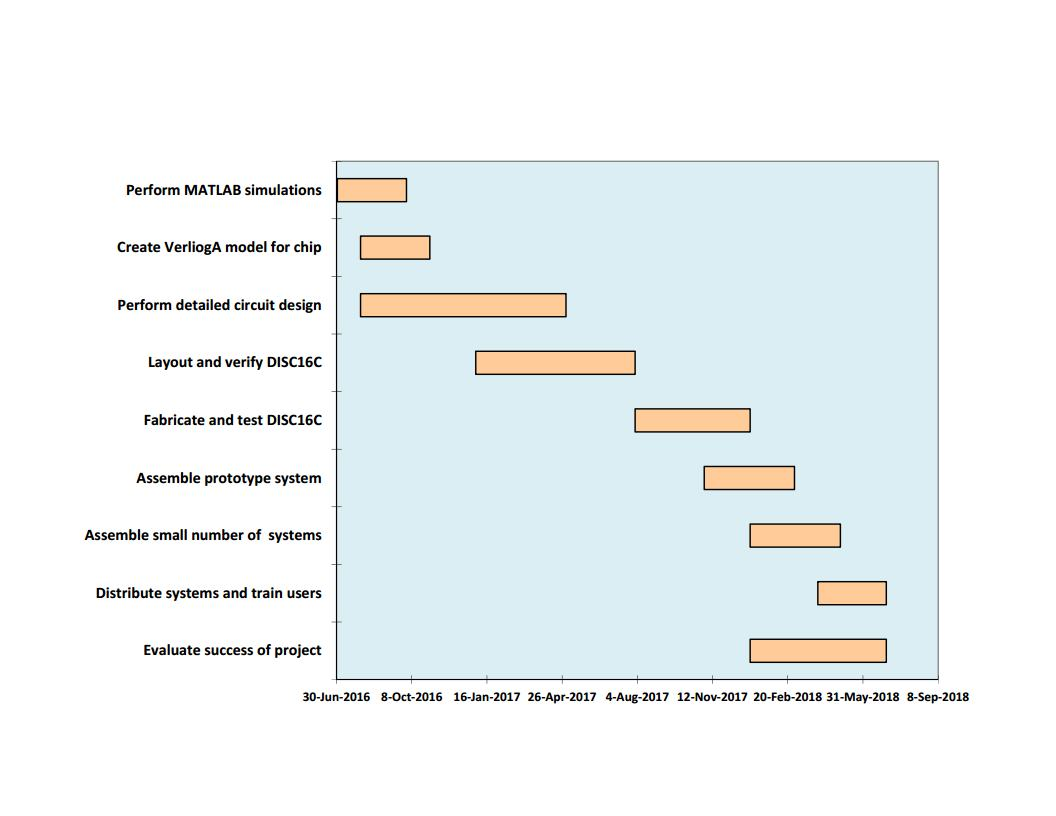
\includegraphics[scale=0.8,keepaspectratio=true, angle=90]{./images/NSFtimeline.jpg}
 	\caption{Timeline of major tasks.}
 	\label{Timeline}
\end{figure}

\section*{Conclusions}

\noindent
The design of a multi-channel discriminator design for a dynamic range from 2 mV to 2 V and rise time constants ranging from 3 ns to 100 ns is feasible. The wide range of pulse risetime constants which must be supported, makes the design challenging but yet quite doable.

\bibliographystyle{IEEEtran}
\bibliography{bibi}

\end{document}